\clearpage
\section{Experiment}
\label{sec:experiment}

We apply our method to the city of Cologne to retrieve insights about how different modes of transport interact and how they contribute to the city's accessibility.
As we want to compare different modes of transport, we will calculate the metric multiple times for different scenarios, each with a different combination of transport modes.
We first introduce each scenario by stating with combination of transport modes it incorporates. 
Next, we present all our sources for the street network data, POIs data, public transport network and schedule data, bicycle sharing data, and land use data.
Lastly, we clearly state all assumptions we make, including the pricing of the different modes.

\subsection{Scenarios}
\label{subs:scenarios}

No matter which mode of transport we choose, we always allow walking for two reasons.
First, walking is the most accessible mode of transport, available to almost everyone and without additional costs.
Second, most other modes of transport require walking at some point, be it to the next bus stop or the next available bicycle.

The first scenario we consider is our baseline, which only includes walking.
This scenario measures what is possible without any additional infrastructure. 
Distinct from other scenarios, it does not require any cost, thus presenting the most basic form of urban mobility.

Building on this, the second scenario we consider is using a personal car.
This scenario depicts the benchmark scenario, as we hope to achieve similar (or even better) results with more sustainable modes of transport.
Travelling by car is highly dependent on traffic and in reality, also requires consideration of the time spent to find parking spots, which is especially impactful in cities.
We disregard parking costs and traffic, and therefore, the resulting times for the car scenario are very optimistic.
This is acceptable as we use the car scenario only as a benchmark.
Therefore, we use it to answer the question of how competitive sustainable modes of transport are compared to the traditional mode of travel by car. 

Transitioning from the benchmark scenario, the third scenario focuses on public transport. 
It is essential to understand the effectiveness and accessibility of urban transit systems. 
This scenario evaluates how well-connected and time-efficient public transportation networks are and their role in reducing reliance on personal vehicles. 
It also investigates the impact of public transport on urban mobility and its potential to contribute to a more sustainable urban environment. 
Specifically, it assesses whether public transport is a viable alternative to the personal car and whether it offers significant advantages over walking, considering the X-minute city metric.
In contrast to the previous scenarios the public transport scenario also incorporates uncertainty.
As the public transport network is scheduled, i.e. time-dependent, we have to consider multiple different starting times, so that we achieve holistic assessment of this mode.

Next, in the fourth scenario, we focus on the dynamics of bicycle-sharing systems. 
This scenario is essential for assessing the feasibility and attractiveness of cycling as a primary mode of transportation in urban areas. 
We will directly compare it to the public transport scenario to understand which sustainable mode of transport is superior.
Similarly to the public transport scenario, we also incorporate uncertainty in this scenario.
The availability of bicycles fluctuates temporally and spatially.
Therefore, we consider multiple different bicycle availability configurations.

Finally, the fifth scenario combines public transport and bicycle sharing, offering insights into the synergy between these two modes of transport.
For brevity, we refer to this scenario as the combined scenario.
This scenario mirrors a growing trend in urban mobility solutions, where multi-modal transport options are increasingly favored. 
We expect it to be the most competitive against cars.

We summarize the scenarios in Table \ref{table:scenarios}.
The specific configuration of the module matrices for each scenario can be found in Appendix \ref{app:experiment_module_matrix_configuration}.

\begin{table}[h]
\centering
\begin{tabular}{|p{4cm}|p{5cm}|p{4cm}|}
\hline
\textbf{Scenario} & \textbf{Modules} & \textbf{Uncertainty} \\
\hline
Walking (baseline) & Walking & - \\
\hline
Personal car (benchmark) & Personal vehicle, walking & - \\
\hline
Public transport & Public transport, walking & Start time \\
\hline
Bicycle sharing & Vehicle sharing, walking & Bicycle availability \\
\hline
Combined & Public transport, bicycle sharing, walking & Start time \& bicycle availability \\
\hline
\end{tabular}
\caption{Scenarios for Urban Mobility Analysis}
\label{table:scenarios}
\end{table}


\subsection{Data}
\label{subs:data}

We require four different datasets to calculate the Pareto sets of our metric for the different scenarios.
First, we require data that depicts the street network of the city of Cologne.
Second, we need to know the locations of the POIs we want to reach.
Third, we need to know the locations of the public transport stops and the schedules of the public transport.
For the bicycle-sharing scenario, we also need to know the locations of the bicycles.
Lastly, we also use land use data to identify where residential areas are located to calculate our metric only for these areas.

As we will query spatial datasets of various formats from different sources, the area covered by the datasets will not be the same.
Therefore, we first define an area of interest and trim the datasets to this area.
In our case, this area is defined as the area of the administrative district of Cologne, specifically the "Stadtkreis Köln".
We retrieve the specific boundary of this area with the help of the Overpass API \shortcite{osm-foundationOverpassAPI2023}.
The specific query can be found in Appendix \ref{app:overpass_query}, and the resulting region can be seen in Figure \ref{fig:area_plus_buffer}.

\begin{figure}
  \begin{center}
    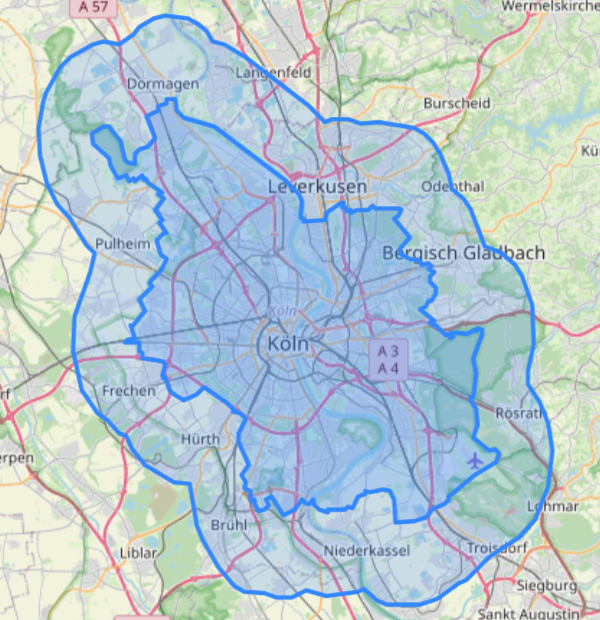
\includegraphics[width=0.55\textwidth]{Figures/experiment/area_plus_buffer.png}
  \end{center}
  \caption{Area of Interest and Buffer Region}\label{fig:area_plus_buffer}
\end{figure}


The Figure additionally depicts a buffer zone surrounding the area of interest.
This expanded area incorporates an additional buffer of approximately 5 km, which is essential as it directly impacts the plausibility of our accessibility analysis.
Specifically, employing a larger underlying street network than the core area of interest circumvents the problem of underestimating accessibility in border regions.

\subsubsection{Street Network \& POIs}
\label{subs:street_network_pois}

For the street network and the POIs, we use data from OpenStreetMap (OSM) \shortcite{osm-foundationOpenStreetMap2023}.
Various tools and services have been developed to use OSM data in practice.
Among these, we use Pyrosm \shortcite{tenkanenPyrosm2023}, a Python library designed specifically for reading OSM data in different formats and conducting data processing operations.
With the help of Pyrosm, we can automatically fetch data from sources like Geofabrik \shortcite{geofabrikGeofabrikDownloadServer2018} and BBBike \cite{schneiderBBBikeExtractsOpenStreetMap2023}, which are two of the most popular OSM data providers.
In our case, we use the data for the city of Cologne from BBBike.
However, due to the flexibility of Pyrosm, it is easily possible to use data from other sources and expand our analysis to other cities.

After retrieving the data, we create a graph representation of the street network trimmed to the buffered area of interest.
Using the buffered region is important because without it, calculating our metric at the border of the area of interest would result in a higher value than the actual value.
To be more specific, we calculate our metric only for regions in the original zone but also use POIs and the street network of the buffered zone.
As the last cleaning step, we remove all nodes not part of the largest weakly connected component.
A weakly connected component is a subgraph in which any two nodes from the subgraph would be connected if all directed edges were treated as undirected.
Multiple weakly connected components in graphs derived from OSM data, mostly happen at the border of the considered area and can be neglected.

Because we consider multiple different modes of transport in the network, it is essential to filter out all edges that are not accessible by the respective mode of transport.
To do so, we use Pyrosm's built-in filtering functionality.
For reproducibility, we list the filters that Pyrosm uses in Appendix \ref{app:pyrosm_network_filter}.

To retrieve the POIs, we use the Overpass API \shortcite{osm-foundationOverpassAPI2023}.
We retrieve all POIs that fall into one of our predefined categories specified in Section \ref{subsec:metric} inside the area of interest plus the buffer mentioned before.

\subsubsection{Public Transport}
\label{subs:public_transport}

We use the General Transit Feed Specification (GTFS) \shortcite{mobilitydataGeneralTransitFeed2023} to handle public transport data.
We rely on the Mobility Database \shortcite{mobilitydataMobilityDatabase2023} to retrieve it.
This database serves as an open-source repository containing links to publicly available GTFS feeds globally.
Similarly to the OSM data, we trim the GTFS data to the area of interest plus the buffer.
The GTFS data is cleaned and converted into a format that is more suitable for McRAPTOR.
Specifically, two significant incompatibilities exist between the GTFS specification and RAPTOR's notion of routes and trips.
Firstly, each trip belonging to a single route in RAPTOR visits the same stops in the same order.
It is impossible for two trips of the same route to use a different sequence of stops.
In GTFS, routes don't pose such restrictions.
For example, two train lines that go along the same set of stops, but in opposite directions, are considered the same route in GTFS.
Secondly, GTFS trips allow visiting the same stop multiple times, which is not permitted in RAPTOR.
To overcome these differences, we split up routes into smaller routes following the same stop sequence.
Additionally, we also remove circular trips altogether, as they only appear in a few cases in Cologne and are not relevant to our analysis.


\subsubsection{Bicycle Sharing}
\label{subs:bicycle_sharing}

Our bicycle-sharing data was retrieved by continuously polling the NextBike API over the course of one year.
The data consists of all trips made with the NextBike system in Cologne from the 15th of January 2022 to the 31st of August 2023.
To get representative samples of the locations of all bicycles, we employ the following strategy.
We first discretize the data spatially and temporally.
For the temporal discretization, we derive the location of each bicycle every hour.
For the spatial discretization, we use H3 hexagons with a resolution of 9.
The resulting data is a set of vectors, where each vector corresponds to a certain hour.
One entry in a vector states how many bicycles are located in the specific hexagon.
This data is then used as an input for k-medoids clustering \shortcite{rdusseeun1987clustering} with a k of 4.
K-medoids, also known as PAM (Partitioning Around Medoids) algorithm, is a clustering technique that partitions a dataset into K clusters, where each is assigned a medoid, the most centrally located object in a cluster. 
Unlike K-means, which uses mean values as cluster centers, K-medoids use an actual data point as the center of a cluster.
This has the advantage that the centers are part of the original dataset, allowing us to retrieve the unaggregated distribution of bicycles for each center.
We use the unaggregated distributions of bicycles of each center as an input for our model.

\subsubsection{Land Use}
\label{subs:land_use}

We utilize the land use data from the CORINE Land Cover (CLC) project \shortcite{european-environment-agencyCORINELandCover2010} to identify the residential areas.
The data covers the whole of Europe and is publicly available, making it possible to expand our analysis to other cities in Europe.
We trimmed the data to the area of interest and then filtered for the land use types "Continuous Urban Fabric" and "Discontinuous Urban Fabric".
These two land use types represent residential areas with different concentrations of residential buildings.
The residential areas inside the area of interest are shown in Figure \ref{fig:input_hexagons_residential_areas}.
Additionally, this Figure shows the hexagons of resolution nine found inside the residential areas.

\begin{figure}
  \begin{center}
    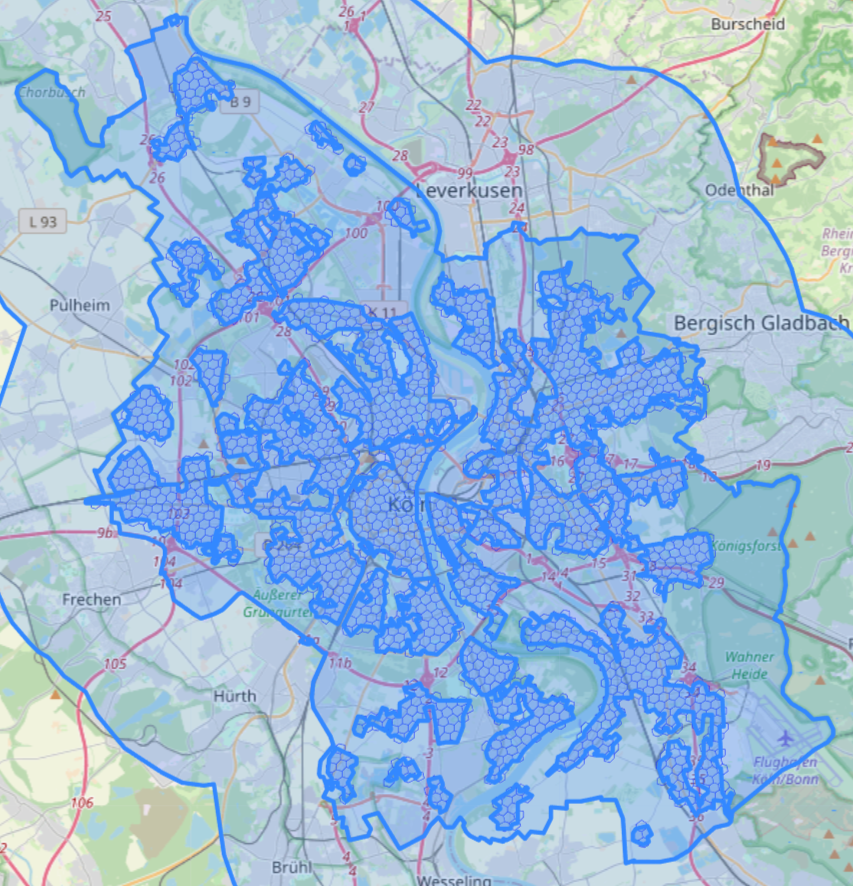
\includegraphics[width=0.65\textwidth]{Figures/experiment/input_hexagons_residential_areas.png}
  \end{center}
  \caption{Area of Interest and Buffer Region with Residential Areas and Input Hexagons}
  \label{fig:input_hexagons_residential_areas}
\end{figure}


\subsection{Assumptions}
\label{subs:assumptions}

To calculate our metric, we have to abstract from reality to some degree.
We do so by making the following plausible assumptions.
 
Firstly, we assume that traveling along an edge of the street network by walking, cycling, or driving is always proportional to the length of the edge, i.e., the travel speed is constant.
To obtain the time it takes to travel along an edge, we divide the length of the edge by the speed of the mode of transport.
The different speeds for the different modes of transport are listed in Table \ref{table:speeds}.

\begin{table}[h]
\centering
\begin{tabular}{|c|l|}
\hline
\textbf{Mode} & \textbf{Speed (m/s)} \\
\hline
Walking & 1.4 \\
\hline
Cycling & 4.0 \\
\hline
Driving & 11.0 \\
\hline
\end{tabular}
\caption{Speeds for Different Modes of Transport}
\label{table:speeds}
\end{table}

The walking speed is consistent with the measurement that \shortciteA{willberg15minuteCityAll2023} made in their study.

We also pose some assumptions on the transitioning between different modes of transport and, in the case of public transport, the transfer time at the stops.
We assume a fixed time of one minute for the transfer time at stops.
To transition from any OSM network-based mode of transport to public transport, we assume that the stop is precisely at the location of the closest node of the OSM network.
As OSM networks contain public transport stops, there should be no difference between the two.
Similarly, we assume that the bicycles are located at the closest node of the OSM network.
This assumption is reasonable because the OSM network, especially in the city, is very dense.
For simplicity, we also assume that bicycles and cars can be parked anywhere on their network.


% \subsubsection{Pricing}
% \label{subs:pricing}
\paragraph{Pricing}

We implement a pricing scheme in our scenarios that represents the real-world circumstances as closely as possible.

For bicycle sharing, we use the pricing scheme of NextBike, which is \euro{1} every 15 minutes.
To depict this, we add a hidden value to the labels processed in MLC that shows how long the current bicycle trip is.
As two consecutive bicycle trips are considered separately, we nullify this hidden value after each run of MLC.

For public transport, we use the pricing scheme of the Cologne Transport Authority (KVB), which is \euro{2.20} for trips that span four stops or less.
For any trip that spans more than four stops or any multitude of trips, the KVB charges \euro{3.20}.
To depict this, we add hidden values to the labels processed in McRAPTOR, representing how many stops the traveler has already traversed.
Because two consecutive trips are considered together, we don't need to nullify the hidden value.

For personal vehicles, we use a cost per minute of \euro{0.19}, which we derived from the average cost per kilometer of \euro{0.28} given by \cite{kieferSpritkostenrechner2023} and an average speed of \SI{40}{\kilo\meter\per\hour}.
These costs incorporate fuel, repair, insurance, and tax, but not acquisition costs.

